\section{Topologische Eigenschaften anhand kritischer Punkte}

Wir wollen die beiden Deformations-Lemmata beweisen, die eine Verbindung zwischen den topologischen
Eingeschaften einer Mannigfaltigkeit und den kritischen Punkten einer Morse Funktion herstellt.
Ist $f \colon M \to \R$ eine glatte Abbildung, dann ist die Subniveaumenge von $f$ bezüglich 
einer reellen Zahl $c$ die Menge $M^c := f^{-1}(- \infty, c]$. Sind $a < b$ reelle Zahlen, dann
stellen die Deformationslemmata die Topologien von $M^a$ und $M^b$ in Relation: Das erste beschreibt, 
was passiert \textit{wenn kein} kritischer Wert überschritten wird, und das zweite beschreibt, was 
passiert \textit{wenn ein} kritischer Wert überschritten wird. Die Beweise folgen Milnors Buch 
\cite{morse}.

\begin{theorem}[Erstes Deformationslemma]
    \label{satz: erstes deformationslemma}
    Es sei $M$ eine glatte Mannigfaltigkeit und $f: M \rightarrow \R$ eine
    glatte Abbildung. Hat $f$ keine kritischen Werte im Intervall $[a, b]$ und 
    ist $f^{-1}[a, b]$ kompakt, so existiert ein Diffeomorphismus 
    $M^a \rightarrow M^b$, und $M^a$ ist ein Deformationsretrakt von $M^b$.
\end{theorem}

Die Idee des Beweises ist es, $M^a$ entlang der Richtung, in die $f$ am stärksten
steigt, also entlang des Gradientenfeldes mit einem Diffeomorphismus $\varphi$ 
"nach oben zu ziehen", bis $\varphi(f^{-1}(a)) = f^{-1}(b)$.
Wir erinnern uns, dass auf jeder Mannigfaltigkeiten \textit{Riemannsche Metriken} existieren,
und dass diese dann für eine Funktion $f \colon M \to \R$ eine Gradientenvektorfeld induzieren.
dieses Gradientenvektorfeld $\grad f$ ist definiert durch 
\[ \langle X , \grad f \rangle = \opd f X \]
und $\grad f (p) = 0$ genau dann, wenn $p$ ein kritischer Punkt von $f$ ist.

\begin{proof}
    Es existiert eine kompakte Umgebung $K \in M$ von $f^{-1}[a, b]$, in der keine kritischen Punkte 
    enthalten sind, das folgt zum Beispiel aus Whitneys Einbettungssatz und dem Satz von Heine-Borel. 
    Sei $\rho: M \to \R$ eine glatte, positive Funktion, sodass
    \[ \rho(p) = 1 / \langle \grad f, \grad f \rangle \]
    für alle $p \in f^{-1}[a, b]$ und die außerhalb von $K$ verschwindet und für
    die für alle $p \in K$, die keine kritischen Punkte sind, gilt: 
    \[ 0 \leq \rho(p) \leq 1 / \langle \grad f, \grad f \rangle \]
    Bemerke dass $\rho$ innerhalb von $K$ wohldefiniert ist, da sich keine kritischen Punkte in $K$ 
    befinden. Definiere ein Vektorfeld $X$ durch
    \[ X(p) = \rho(p) \cdot \grad f (p) \]
    Dann hat $X$ kompakten Träger, erfüllt also die Vorraussetzungen von 
    Lemma~\ref{prop: kompaktes VF generiert 1-param. grp.}. Sei also $\varphi$ die
    einzigartige 1-Parameter Gruppe aus Diffeomorphismen, die von $X$ generiert
    wird. 
    Wir bekommen für jedes $p \in M$ eine Abbildung 
    $f \circ \varphi_{\bullet}(p): \R \to \R$.
    
    \begin{claim*} 
        Für alle $p \in M$, $t_0 \in \R$ und $q = \varphi_{t_0}(q)$
        ist $\derive{t} f \circ \varphi_{\bullet}(p) (t_0) \in [0, 1]$ und falls 
        $f(\varphi_t(q)) \in [a, b]$ gilt sogar $\derive{t} f \circ \varphi_{\bullet}(q) (t_0) = 1$.
    \end{claim*}

    \begin{smallproof}
        Für $q = \varphi_{t_0}(p)$:
        \begin{align*}
            \derive{t} f \circ \varphi_{t_0}(p)
            & = \opd f (\varphi_{t_0}(p)) \cdot \opd \varphi_{\bullet}(p) (t_0) 
                \left( \derive{t} \right)
            = \opd f (q) \cdot X(q) \\
            & = \langle X(q), \grad f (q) \rangle 
            = \rho(q) \langle \grad f (q), \grad f (q) \rangle \in [0, 1]
        \end{align*}
        $f \circ \varphi_{\bullet}(p)$ ist also monoton wachsend für alle $p \in M$.
        Falls sogar $f(\varphi_p(t_0)) \in [a, b]$, dann gilt
        \[ \frac{d}{dt} f \circ \varphi^p (t_0) = 1 \]
    \end{smallproof}

    Man zeigt dann leicht, dass für $p \in f^{-1}(a)$, $t_0 \in [0, b-a]$ gilt 
    $f(\varphi_{t_0}(p)) \in [a, b]$.

    Dann ist für $p \in f^{-1}(a)$ die Abbildung $f \circ \phi_{bullet}(p)$ im Intervall $[0, b - a]$
    linear mit Steigung $1$ und es gilt 

    \[ f(\varphi_{b - a}(p)) = f(\varphi_{0}(p)) + (b - a) = b \]
    Genauso für $q \in f^{-1}(b)$: $f(\varphi_{a - b}(q)) = a$, also 
    $\varphi_{b - a}(f^{-1}(a)) = f^{-1}(b)$.

    Dann haben wir $\varphi_{b - a} (M^a) = M^b$, also ist $\varphi_{b - a}|_{M^a}$ ein 
    Diffeomorphismus zwischen $M^a$ und $M^b$. 

    Betrachte nun $r: M^b \times \R \to M^b$,
    \[  
        r(p, t) = \begin{cases}
            p & \text{ falls } f(p) \leq a \\
            \varphi_{t(a - f(p))}(p) & \text{ falls } a \leq f(p) \leq b 
        \end{cases}
    \]

    $r$ ist stetig, $r(\cdot, 0)$ ist die Identität auf $M^b$, 
    $r(\cdot, 1)|_{M^a}$ ist die Identität auf $M^a$ und 
    $r(1, M^b) \subseteq M^a$, also ist $M^a$ ein Deformationsretrakt von $M^b$.
\end{proof}

\begin{theorem}[Zweites Deformations-Lemma]
    \label{satz: zweites deformationslemma}
    Es sei $M$ eine glatte Mannigfaltigkeit, $f: M \rightarrow \R$ eine glatte
    Abbildung und $p$ ein nicht-degenerierter kritischer Punkt mit Index 
    $k$. Sei $c := f(p)$ und $\varepsilon \geq 0$, sd. 
    $f^{-1}[c - \varepsilon, c + \varepsilon]$ kompakt ist und außer $p$ keine 
    weiteren kritischen Punkte von $f$ beinhaltet. Dann hat $M^{c-\varepsilon}$
    denselben Homotopietypen wie $M^{c - \varepsilon} \cup e^k$.
\end{theorem}

\begin{proof}
    Die Idee für den Beweis ist, sich eine neue Funktion $F: M \to \R$ zu definieren,
    die Außerhalb von einer kleinen Umgebung von $p$ $f$ entspricht und in der 
    Umgebung etwas kleiner ist. Dann bekommen wir die folgende Situation:

    \begin{figure}[H]
        \centering
        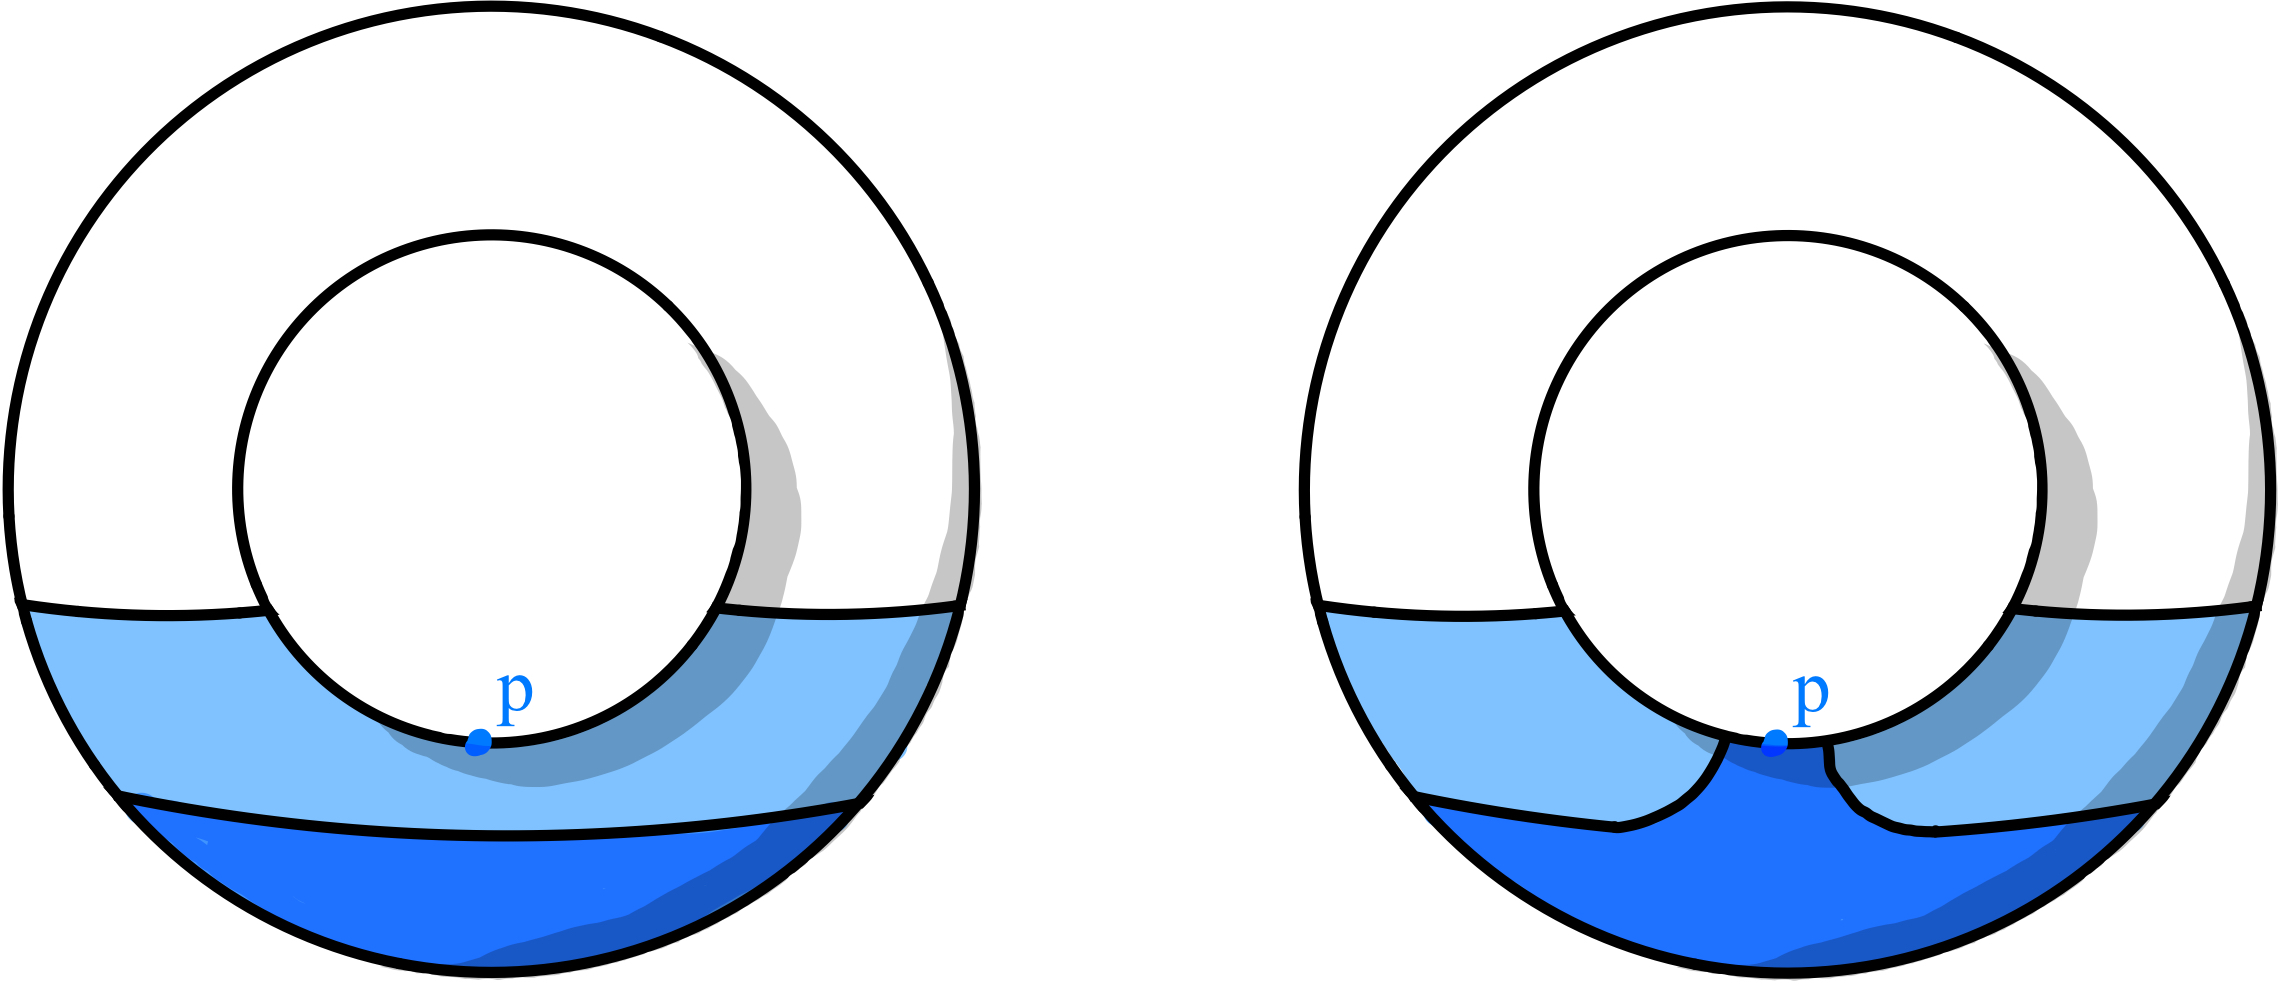
\includegraphics[width=0.8\linewidth]{../resources/Me-Diagram5-sublevelsets-of-f-and-F.jpeg}
        \label{fig:me-diagram5}
        \caption{Die Niveaumengen von $f$ (links) und $F$ (rechts)}
    \end{figure}

    Wir wollen also, dass $M^{c + \varepsilon} = F^{-1}(- \infty, c + \varepsilon]$ 
    gilt und $F^{-1}(-\infty, c - \varepsilon]$ fast dasselbe ist wie 
    $M^{c - \varepsilon}$, nur dass $F^{-1}(-\infty, c - \varepsilon]$ einen "Henkel"
    enthält der den kritischen Punkt $p$ enthält.

    Wir benutzen das Morse-Lemma~\ref{satz: morse-lemma}:
    Wir finden lokale Koordinaten $\phi = (u_1, \dots, u_n)$ in einer Umgebung $U$ von $p$, sodass 
    \[ f = c - u_1 - \dots - u_k + u_{k + 1} + \dots + u_n \]
    und
    \[ u_1 (p) = \dots = u_n(p) = 0 . \]
    Sei $\eps$ ohne Beschränkung der Allgemeinheit klein genug, sodass $f^{-1}[c - \eps, c + \eps]$ 
    kompakt ist und die Kreisscheibe $\{ x \in \R^n : \| x \|^2 \leq 2 \eps \}$ im Bild von $\phi$ 
    enthalten ist. Wähle nun die $k$-Zelle 
    \[ e^k := \{ q \in M : u_1^2 (q) + \dots + u_k^2 (q) \leq \eps \text{ und }
        u_{k + 1} (q) = \dots = u_n (q) = 0 \} . \]
    Wir bekommen folgende Situation:
    \begin{figure}[H]
        \centering
        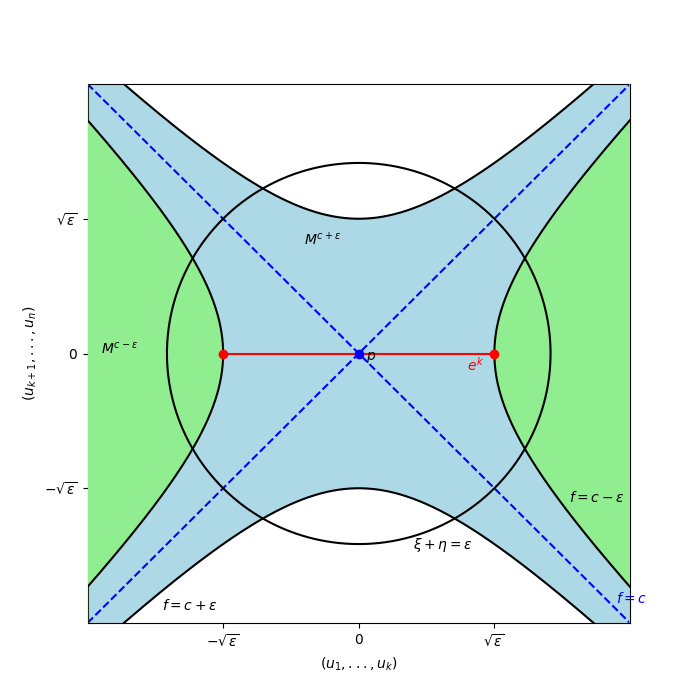
\includegraphics[width=0.45\linewidth]{../resources/Me-Diagram6-U-parameterized.png}
        \label{fig:me-diagram6}
    \end{figure}
    $F$ wird nun so definiert, dass eine Umgebung der $k$-Zelle $e^k$ ein wenig abgesenkt wird.
    Sei $\mu \colon \R \to \R$ eine glatte Funktion mit den Eigenschaften
    \begin{enumerate}
        \item $\mu(0) > \eps$
        \item $\mu (r) = 0$ falls $r \geq 2 \eps$
        \item $-1 < \mu' (r) \leq 0$ für alle $r \in \R$ .
    \end{enumerate}
    Sei dann $F$ außerhalb von $U$ gleich $f$, und innerhalb von $U$ setze
    \[ F = f - \mu ( u_1^2 + \dots + u_k^2 + 2 u_{k + 1}^2 + \dots + 2 u_n^2) . \]
    Man überprüft dann die drei Behauptungen
    \begin{enumerate}
        \item $F^{-1}(- \infty, c + \eps] = M^{c + \eps}$,
        \item $F^{-1}(- \infty, c - \eps]$ ist Deformationsretrakt von $M^{c + \eps}$,
        \item $M^{c - \eps \cup e^k}$ ist Deformationsretrakt von $F^(- \infty, c - \eps]$.
    \end{enumerate}
    Die zweite Behauptung folgt aus dem ersten Deformationslemma.
    
    Den detaillierten Beweis findet man zum Beispiel in \cite{milnor}.
\end{proof}

Mit diesen beiden Aussagen kommt man schon sehr weit. Die berühmten Morse- \\Ungleichungen lassen
sich mit ein bisschen linearer Algebra an exakten Sequenzen leicht daraus folgern. Man kann sogar
zeigen, dass jede Mannigfaltigkeit dein Homotopietypen eines CW-Komplexes 
(siehe Def.~\ref{def: cw-komplex}) besitzt, wie es zum Beispiel Milnor tut. Die folgenden Kapitel 
geben eine etwas eleganterere Sicht auf die Thematik, die in gewisser Hinsicht stärkere Aussagen
liefert:

\textit{Kompakte} Mannigfaltigkeiten haben nicht nur den selben Homotopie-Typen eines CW-Komplexes, 
sondern sie sind sogar CW-Komplexe, und wir können uns die zelluläre Homologie, die aus der 
CW-Struktur hervorgeht sogar auf eine einfache Art und Weise erklären.